% arara: pdflatex: { synctex: yes }
% arara: makeindex: { style: ctuthesis }
% arara: bibtex

% The class takes all the key=value arguments that \ctusetup does,
% and a couple more: draft and oneside
\documentclass[twoside]{ctuthesis}

\ctusetup{
%	preprint = \ctuverlog,
	mainlanguage = english,
	titlelanguage = english,
%	mainlanguage = czech,
	otherlanguages = {czech,english},
	title-czech = {Rádiové určování polohy letících objektů},
	title-english = {Radio Position Determination of Flying Objects},
%	subtitle-czech = {Cesta do tajů kdovíčeho},
%	subtitle-english = {Journey to the who-knows-what wondeland},
	doctype = D,
	doctype-czech = Obhajoba minima,
    doctype-english = Thesis proposal, % or whatever
	faculty = F3,
	department-czech = {Katedra měření},
	department-english = {Department of Measurement},
	author = {Jakub Kákona},
	supervisor = {Doc. Dr. Ing. Pavel Kovář},
	supervisor-address = {Department of Radio Engineering},
%	supervisor-specialist = {John Doe},
	fieldofstudy-english = {Air Traffic Control},
	subfieldofstudy-english = {Radio navigation},
	fieldofstudy-czech = {Provoz a řízení letecké dopravy},
	subfieldofstudy-czech = {Rádiová navigace},
	keywords-czech = {Radar, GRAVES, meteor, výpočet trajektorie metoru },
	keywords-english = {Multi-static radar system, meteor, GRAVES, trajectory estimation},
	day = 2,
	month = 5,
	year = 2017,
%	specification-file = {ctutest-zadani.pdf},
%	front-specification = true,
	front-list-of-figures = false,
	front-list-of-tables = false,
%	monochrome = true,
%	layout-short = true,
	savetoner = false,
}



\ctuprocess

\addto\ctucaptionsczech{%
	\def\supervisorname{Vedoucí}%
	\def\subfieldofstudyname{Studijní program}%
}

\ctutemplateset{maketitle twocolumn default}{
	\begin{twocolumnfrontmatterpage}
		\ctutemplate{twocolumn.thanks}
		\ctutemplate{twocolumn.declaration}
		\ctutemplate{twocolumn.abstract.in.titlelanguage}
		\ctutemplate{twocolumn.abstract.in.secondlanguage}
		\ctutemplate{twocolumn.tableofcontents}
		\ctutemplate{twocolumn.listoffigures}
	\end{twocolumnfrontmatterpage}
}

% Theorem declarations, this is the reasonable default, anybody can do what they wish.
% If you prefer theorems in italics rather than slanted, use \theoremstyle{plainit}
\theoremstyle{plain}
\newtheorem{theorem}{Theorem}[chapter]
\newtheorem{corollary}[theorem]{Corollary}
\newtheorem{lemma}[theorem]{Lemma}
\newtheorem{proposition}[theorem]{Proposition}

\theoremstyle{definition}
\newtheorem{definition}[theorem]{Definition}
\newtheorem{example}[theorem]{Example}
\newtheorem{conjecture}[theorem]{Conjecture}

\theoremstyle{note}
\newtheorem*{remark*}{Remark}
\newtheorem{remark}[theorem]{Remark}

\setlength{\parskip}{5ex plus 0.2ex minus 0.2ex}


% Only for testing purposes
\listfiles
\usepackage[pagewise]{lineno}
\usepackage{lipsum,blindtext}
\usepackage{mathrsfs} % provides \mathscr used in the ridiculous examples

\begin{document}

\maketitle

\chapter{Motivation}
Radio position determination of flying objects is a key radiolocation discipline which allows safe operation of aircraft and spaceships. The radar systems developed in last decades have enough properties to solve standard situations \cite{Radar_basics}. However, some safety problems related to unusual conditions are not resolved yet \cite{lightning_dose1}. These situations could be caused by extremal weather events like thunderstorms for example, where lightning can damage an airplane or limit a radio communication and navigation capabilities in affected area \cite{lightning_dose2}. Additionally, according to recent scientific discoveries, lightning discharges can produce an ionizing radiation which could significantly enhance an effective dose of aircraft crew and passengers \cite{lightning_dose3}, \cite{lightning_dose4}, \cite{lightning_dose6}. 
Therefore a research which helps quantify, predict and avoid these hazards should improve overall air traffic safety \cite{lightning_dose5}. This goal should be achieved by improving understanding of unusual atmospheric events and enhance sensing capabilities in extreme circumstances. 
Unfortunately, hazardous conditions can have multiple different forms with different suitable detection methods which should often be combined to produce a desirable result, but at least for some cases, a radar sensing system should be a suitable option. 
The parameters of that detection system should be universal as possible and assume possible combination with other detection methods. 
However, in opposite to that the common technique, for natural phenomena detection is building an experiment-specific radar system. 
This approach is shown in scientific papers, which describe state of the art radio detection methods of natural phenomena. For example, a lightning detection systems like \cite{NMLMA} uses specifically designed direction finding and time measurement receiver system.  Another system is intended to be a meteor scatter receiver on the specific frequency and position \cite{BRAMS}. 
By combining parameters required by these and possibly other systems, a universal receiver useful for multi-experiment natural object detection could be built. The source \cite{LOFAR} describes the first and extremely expensive solution for this problem. The LOFAR station design and requirements are prohibitive for widespread scientific use, but a use of new techniques could scale down the station complexity and allows a small scale high-quality radio experiments which should help to improve the knowledge about atmospheric processes. Then the proper methods and algorithm should be developed to discover evidence of hazardous conditions and suggest appropriate steps to improve safety. 

\section{Main object parameters}

The radar cross section (RCS; describing the ability to reflect radio waves), object distance and velocity are typical limiting parameters of the radar systems. These parameters vary largely depending on the measured target type and limit overall energy budget of the radar system. Therefore main groups of objects which should emerge in airspace will be described separately. 

\subsection{Artificial airspace targets}

A large group of possible radio reflective targets includes classical airspace objects like airplanes, unmanned aerial vehicles or satellites. These classical objects are detectable and localizable with already existing radar systems. Parameters like RCS and trajectory or velocity of these object are usually known from other sources simultaneously, and therefore this object category is usable for system parameters' verification. Otherwise, these objects are typically treated as noise in scientific measurements. 

\subsection{Natural radio-detectable objects}

Several natural atmospheric or near space phenomena are expected to be localized by radio-waves. The list, for example, contains Solar system bodies, meteors, ionospheric fluctuations, solar flares, cosmic rays' particles and atmospheric electrical discharges. Not all of these natural phenomena have confirmed radio detection due to technical limitations or yet unknown physical principles \cite{LOPES}, \cite{astro_particles}, \cite{LOFAR_showers}.

\subsubsection{Reflective objects}
A radio signal source should illuminate the objects which do not radiate signal itself. 
The one of oldest known radio detection method such object type is a backscatter radar. It is an ordinary type of radar which expects reflective targets and illuminating them by radio signal which is transmitted from almost the same place as a receiver is located. Currently, several radars of this type are in operation to study meteors i. e.  SkiYMet\cite{skiymet}, CMOR \cite{CMOR_radar}.

Meteors, the atmospheric products of meteoroids traveling in space, are studied for many decades \cite{interplanetary_medium}. As the density of the interplanetary medium is low, great statistic and long-term continuous data set is necessary to describe meteor properties and measure an exact density of impacts.

However, all mentioned  \cite{skiymet},\cite{CMOR_radar}  monostatic or bistatic backscatter radars have little detection coverage, usually limited to the radar antenna field of view. Therefore these radar types observe only several spatially limited areas of the Earth's atmosphere.
Besides the backscatter scientific radar systems, a multistatic forward scatter radio meteor detection networks have evolved \cite{BRAMS},\cite{RETRAM}.
The general principle of meteor observing by the forward scattering of radio waves off their trails is illustrated by the figure \ref{fig:forward_scattering}. A radio receiver with operating frequency range of 30-200MHz is located at a proper distance (about 500-2000 km) from a transmitter. A curvature of the Earth or terrain features over this distance ensures there is no possibility of direct radio visibility. When a meteoroid enters the atmosphere, its meteor trail may reflect the radio waves emitted by the transmitter to the receiver. The signal can be received until the ionized meteor trail recombines. Reflections can last from tenths of a second to a few minutes, depending on the used radio frequency and ionization density. The received signal characteristics are directly related to physical parameters of the meteoric event \cite{forward_scatter}.

These forward scattering multistatic systems have a great advantage of a significant detection coverage. 
The main improvement of coverage, which the forward scattering method brings, originate in the fact that one or multiple radio-frequency transmitters can be cooperatively handled simultaneously over the large area. Additionally, forward scattering geometry decreases the angle of reflection, therefore increased frequency of the transmitter can be used. Unfortunately, the current spread of this technology is not sufficient to entirely cover the meteor flux in the Earth's atmosphere.
However, the benefits of using this radio method are obvious - radio meteor detection capability is not dependent on the current weather and can work even during the daylight or nights with full Moon \cite{daylight_shover}.

\begin{figure}
 \begin{center}
 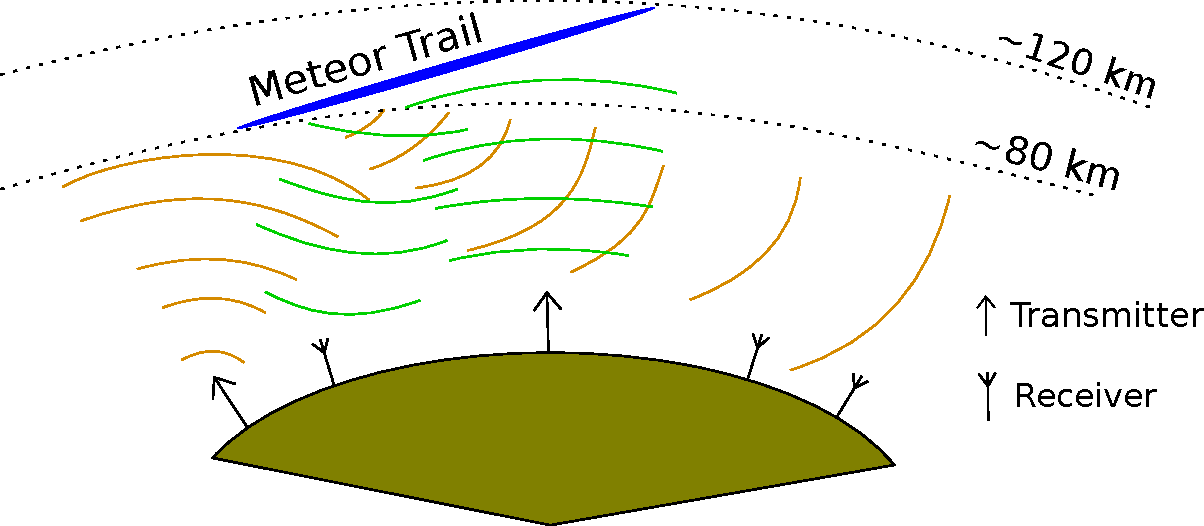
\includegraphics[width=\linewidth]{./img/Meteor_detection.pdf}
 \caption{The method of radio meteor detection based on the forward scattering radar system}
  \label{fig:forward_scattering} 
 \end{center}
\end{figure}

\subsubsection{Emissive objects}

Another object detection principle relies on the fact that some phenomena are radio emissive targets itself. A typical example of such object is thunderstorm lightning. The lightning detection and localization stations work on VLF, LF, and VHF radio bands. Selected frequency and bandwidth depend on the application of the system. The long range lightning surveillance systems use VLF frequencies. Essentially all methods that provide accurate information about the location,  polarity,  and peak current of return strokes in the cloud to ground, lightning operates in this frequency range. This sensor type usually extracts a basic signal feature like time of trigger and amplitude by preset of waveform discrimination criteria \cite{VLF_TOGA}. Then the measured time and possible azimuth of received signal of the event from multiple stations is processed in the central processing unit. The signal source is assumed to be point-like; therefore the spatial resolution of the best implementations of this technique are limited to sub-kilometer precision \cite{Lightning_locating}. 
For more precise measurement a shorter wavelength from VHF band is used, where a combination of time of arrival and interferometry methods are preferred for reconstructing lightning channel \cite{NALMA_algorithms}, \cite{rocket_triggered}. 

The newer detection systems are exclusively based on proprietary Vaisala  IMPACT \cite{IMPACT_sensor} or TLS200/TSS928/LS7002 lightning sensors. 
Furthermore commercial off the shelf products are preferred systems for long-term sustainability \cite{4DLSS}. Unfortunately, these systems are intended to be used in meteorological measurements and insured events solving. Therefore they are not suitable for research of atmospheric phenomena. The only one exception to this trend I have found in the literature is lightning research which takes place in LOFAR project \cite{LOFAR_lightning}, \cite{LOFAR_lightning2}.  

\section{Common position determination methods}

If we want to estimate target position by radio signal reflected or transmitted by the target, we have only a small number of signal features which we could use to obtain the information about target coordinates. The best method to be used for determination of target position depends on the target type, the measurement precision required and intended application. In most cases for an unknown flying object, we need to implement and combine several of the following general methods. 

\subsection{Direction finding}

Radio direction finding is the oldest radio localization method.  It uses receiver system sensitive to the angular orientation of the incoming signal.  The target is then localized by combining angular information from multiple receivers.  The direction sensitivity of a system was historically achieved by using a directional antenna. Nowadays the system usually uses antenna arrays consisting of antenna elements with a semi-omnidirectional radiating pattern. Then the received signal direction is numerically calculated from phase shift differences of the signal received by the antenna array. Several algorithms exist to calculating target position from the angle of arrival measurement (AOA) the one of latest is Robust Weighted Intersection Algorithm from the source \cite{RWIAOA}. The AOA value can be theoretically calculated from the simplest two element antenna array according to equation \ref{AOA_Angle}. Unfortunately, the calculated $\Theta$ is ambiguous AOA. Therefore more complex antenna arrays are used for serious measurements \cite{Interferometry_AOA}.  

\begin{equation}
 \Theta = \arcsin \left( \frac{\Delta \phi \lambda}{2 \pi  d} \right)
 \label{AOA_Angle}
\end{equation}

\subsection{Distance measurement}
Localizing a target by radio distance measurement usually uses the time-variable radio signal, rarely a signal attenuation model.  The target position is obtained by combining measured distances between the target and the receiver using geometrical trilateration or multilateration. The general limiting factor of this method is the requirement of a time-space variance of the radio signal which could not be achieved in every case. 
In some cases, a pulse signal could be used for distance measurement. This technique is used in almost all existing lightning localization networks. The distances are obtained by measurement of time of arrival (TOA) or time of group arrival (TOGA) respectively.

To determine the 3-dimensional structure and temporal development of a lightning discharge the most systems utilizes the basic technique employed by the lightning mapping array (LMA) that has been developed and operated at Kennedy Space Center by Carl Lennon and Launa Maier. The LMA uses time of arrival measurements to locate impulsive VHF radiation events during discharge. The figure \ref{fig:lihting_discharge} shows the VHF signal for a portion of a normal lightning discharge. The sharp peaks in the plotted signal are produced by impulsive electrical breakdown events in small source regions \cite{NMLMA}. The detection method of the transient peak in the band-limited signal in the presence of noise directly affect the measurement quality \cite{Transient_peak}. 

\begin{figure}
 \begin{center}
 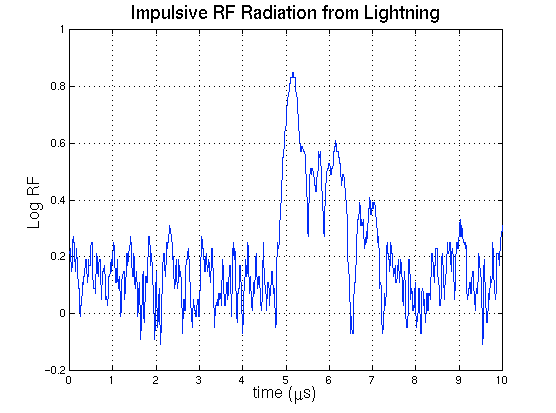
\includegraphics[width=\linewidth]{./img/lightning_waveform.png}
 \caption{Hilbert envelope of a lightning discharge signal. Source: \cite{NMLMA} }
  \label{fig:lihting_discharge} 
 \end{center}
\end{figure}

If the time of arrival of the radiation from such an event is measured at four locations, the 3-dimensional position of the source region can be determined. If impulsive radiation occurs at location ($x$, $y$, $z$) and at time $t$, the time it is received at station i is 

\begin{equation}
t_i = t+ \frac{sqrt( (x-x_i)^2 + (y-y_i)^2 +(z-z_i)^2)}{c} \label{toa}
\end{equation}

where ($x_i$, $y_i$, $z_i$) is the position of station $i$. 

\begin{figure}
 \begin{center}
 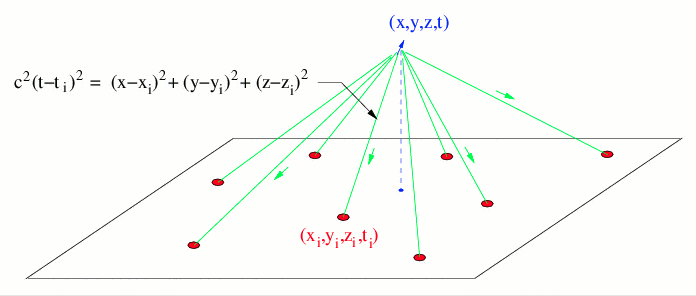
\includegraphics[width=\linewidth]{./img/toa_fig.png}
 \caption{Illustration of measured distances in TOA methods. Source: \cite{NMLMA} }
  \label{fig:TOA_localization} 
 \end{center}
\end{figure}

By measuring the time of arrival of the radiation at least a four stations the four unknowns (x,y,z,t) can be determined. To provide for redundancy in the data (so a noise spike at one of the stations is not misidentified as a source of lightning) the system uses multiple receivers. The data from all stations is used to determine the location (and error in location) of the radiation source \cite{NMLMA}.

\subsection{Velocity measurement}

The key principle is a bistatic Doppler shift described by equation \ref{bistatic_doppler}. The method is based on the fact that multiple receivers receiving the same signal reflected or generated by the same target have seen different Doppler shifted signal depending on the velocity vector of the target.  

\begin{equation}
f = \frac{1}{\lambda} \frac{d}{dt} \left( R_{tx} + R_{rx} \right)
\label{bistatic_doppler}
\end{equation}

Where 
\begin{itemize}
\item $f$ - Received frequency
\item $\lambda$ - Radar transmitter operating frequency wavelength in meters
\item $R_{tx}$ - Distance between the transmitter and the target
\item $R_{rx}$ - Distance between the receiver and the target.
\end{itemize}

This method can localize only moving targets, but it is especially suitable for fast airspace targets which could not stop their movement due to physical laws restrictions. 

\chapter{Experimental verification}

The following section describes a real experimental work, which was carried out to verify the natural phenomena detection hypotheses described above. The experimental universality of the developed system was implemented wherever possible. 

\section{Meteor detection system}

Meteors were selected primarily as the core natural objects testing phenomenon because they have unusual properties like high velocities and a wide range of RCS.
Proposed Bolidozor network \cite{Bolidozor} uses multistatic forward scattering approach which allows an efficient use of the radar transmitter energy to maximize the information value collected from the meteor reflection.
The network currently uses GRAVES \cite{GRAVES_radar} transmitter located in France, which transmits a continuous wave (CW) signal at a frequency of 143.05 MHz. A radiation of the transmitter is directed mainly to the south hemisphere, but due to the imperfections of its antenna system, the signal from meteor reflections can be observed in almost all European countries. Therefore the transmitter is suitable for receivers' network operations with the aim of meteor trail detection and the development of algorithms for the calculation of meteor trajectory. Unfortunately, the use of a distance measurement method is not possible because the transmitter signal is only partially modulated in space by steering the transmit azimuth in several discrete sectors, but the exact method and timing of steering radar beam we can not control. 

\begin{figure}
 \begin{center}
 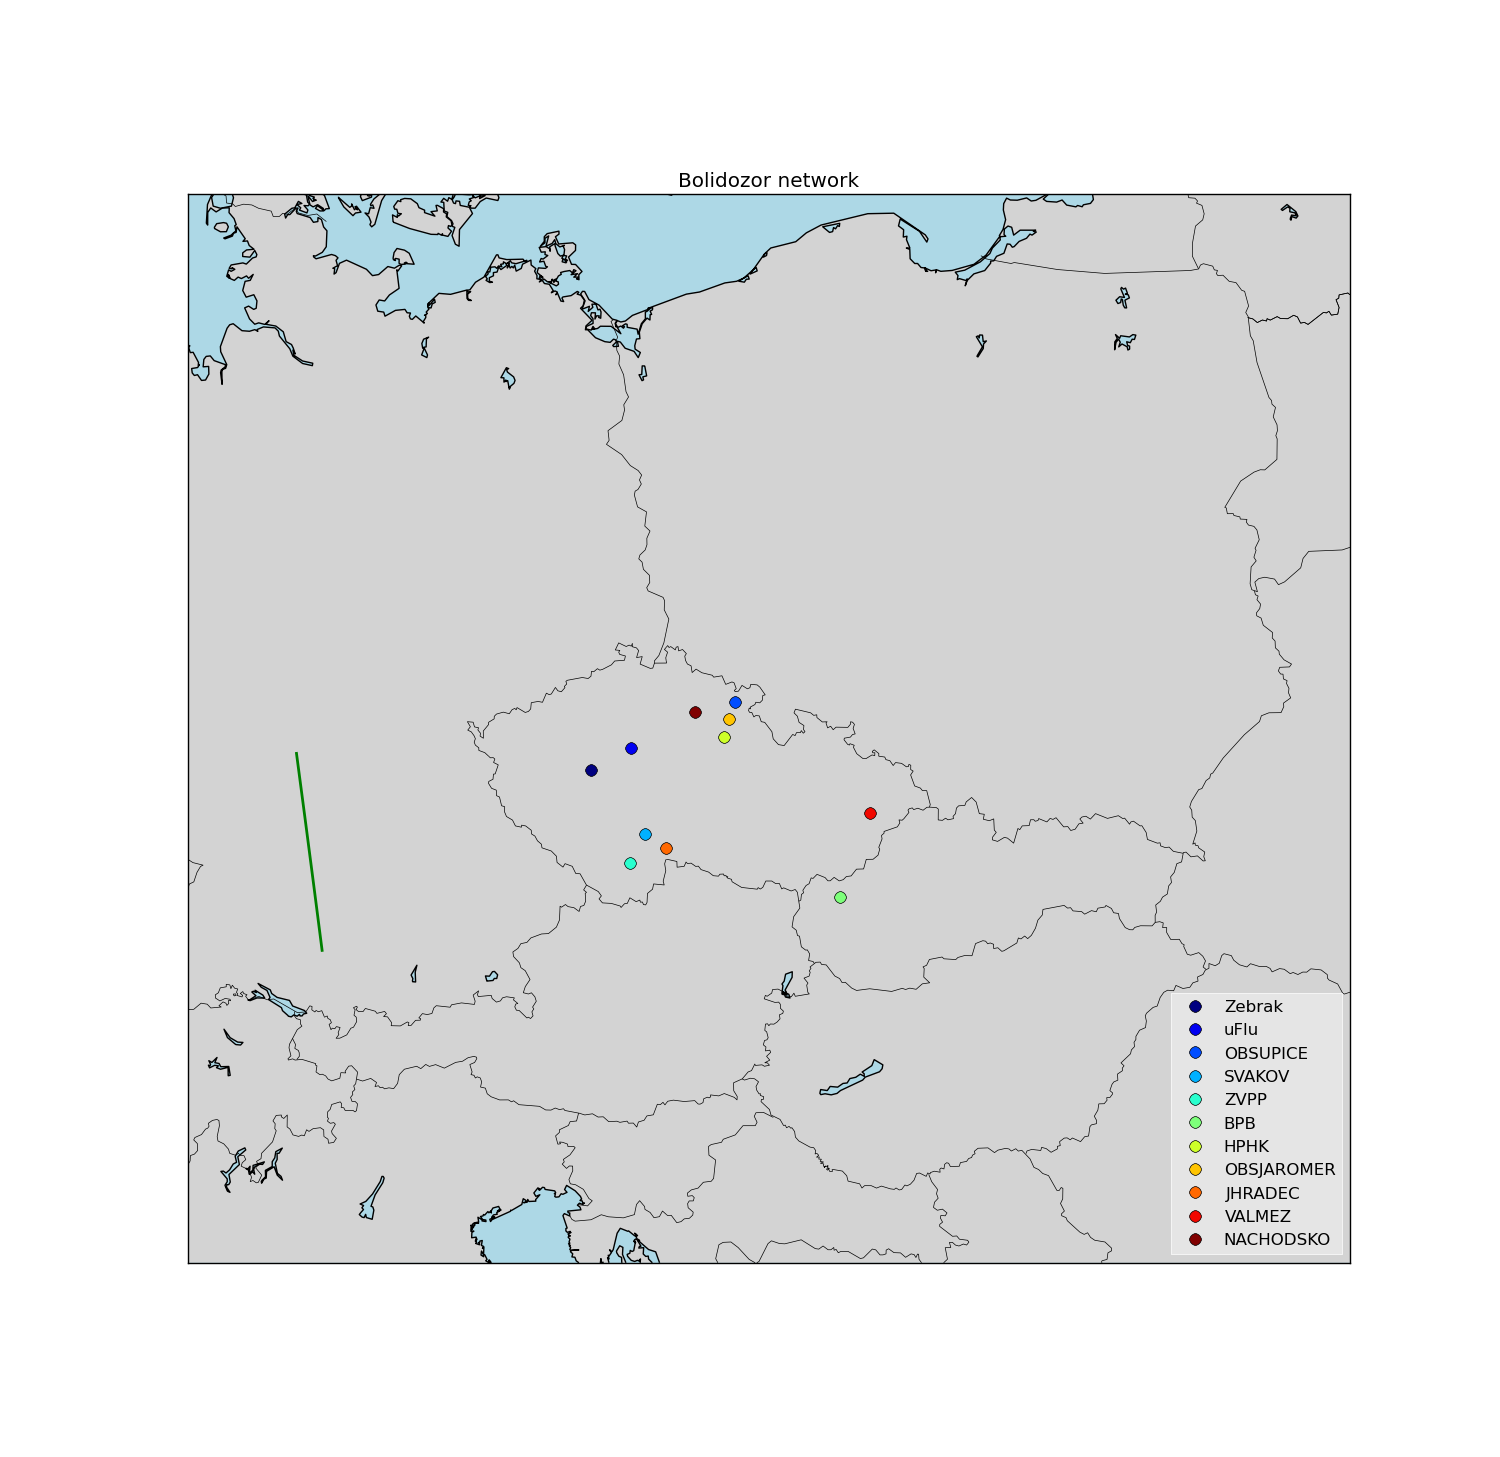
\includegraphics[width=\linewidth]{./img/stanice_mapa.png}
 \caption{Bolidozor stations network}
  \label{fig:stanice_mapa} 
 \end{center}
\end{figure}
                   
The use of such high-frequency beacon has one main advantage over the previous meteor detection experiments.
Previous attempts used longer radio wavelengths in frequency range 20-50 MHz. Such long wavelengths were used to obtain a higher sensitivity to finer meteor trails. According to a simplified formula (\ref{equ:decay}), where $T$ is the exponential time constant and $D$ is ambipolar diffusion coefficient and $\lambda$ is wavelength \cite{Decay_time}. The equation implies that at longer wavelengths we observe the meteor's echo for a longer period of time compared to shorter wavelengths. However, shorter wavelengths allow us to detect finer details of meteor trails.

\begin{equation}
T = \frac{\lambda^2}{16 \pi ^2 D}
\label{equ:decay}
\end{equation}

The head echo of a meteor is usually called overdense plasma due to its relatively high plasma frequency compared to used observation frequency ($F_{obs}$) in the front of the meteoroid shock wave that is created in the air. This condition is expressed by the equation (\ref{equ:plasma_frequency}). However, if we use a frequency close to the plasma frequency ($f_{pe}$) of the meteor trail, we can distinguish the head echo and the meteor trail reflection because the Doppler shift is applied on the part of the reflected signal. This situation is shown in the figure \ref{fig:meteor_reflections} where sloped dotted lines mark head echoes. Straight vertical lines indicate static meteor trail reflections.

\begin{figure*}
 \begin{center}
 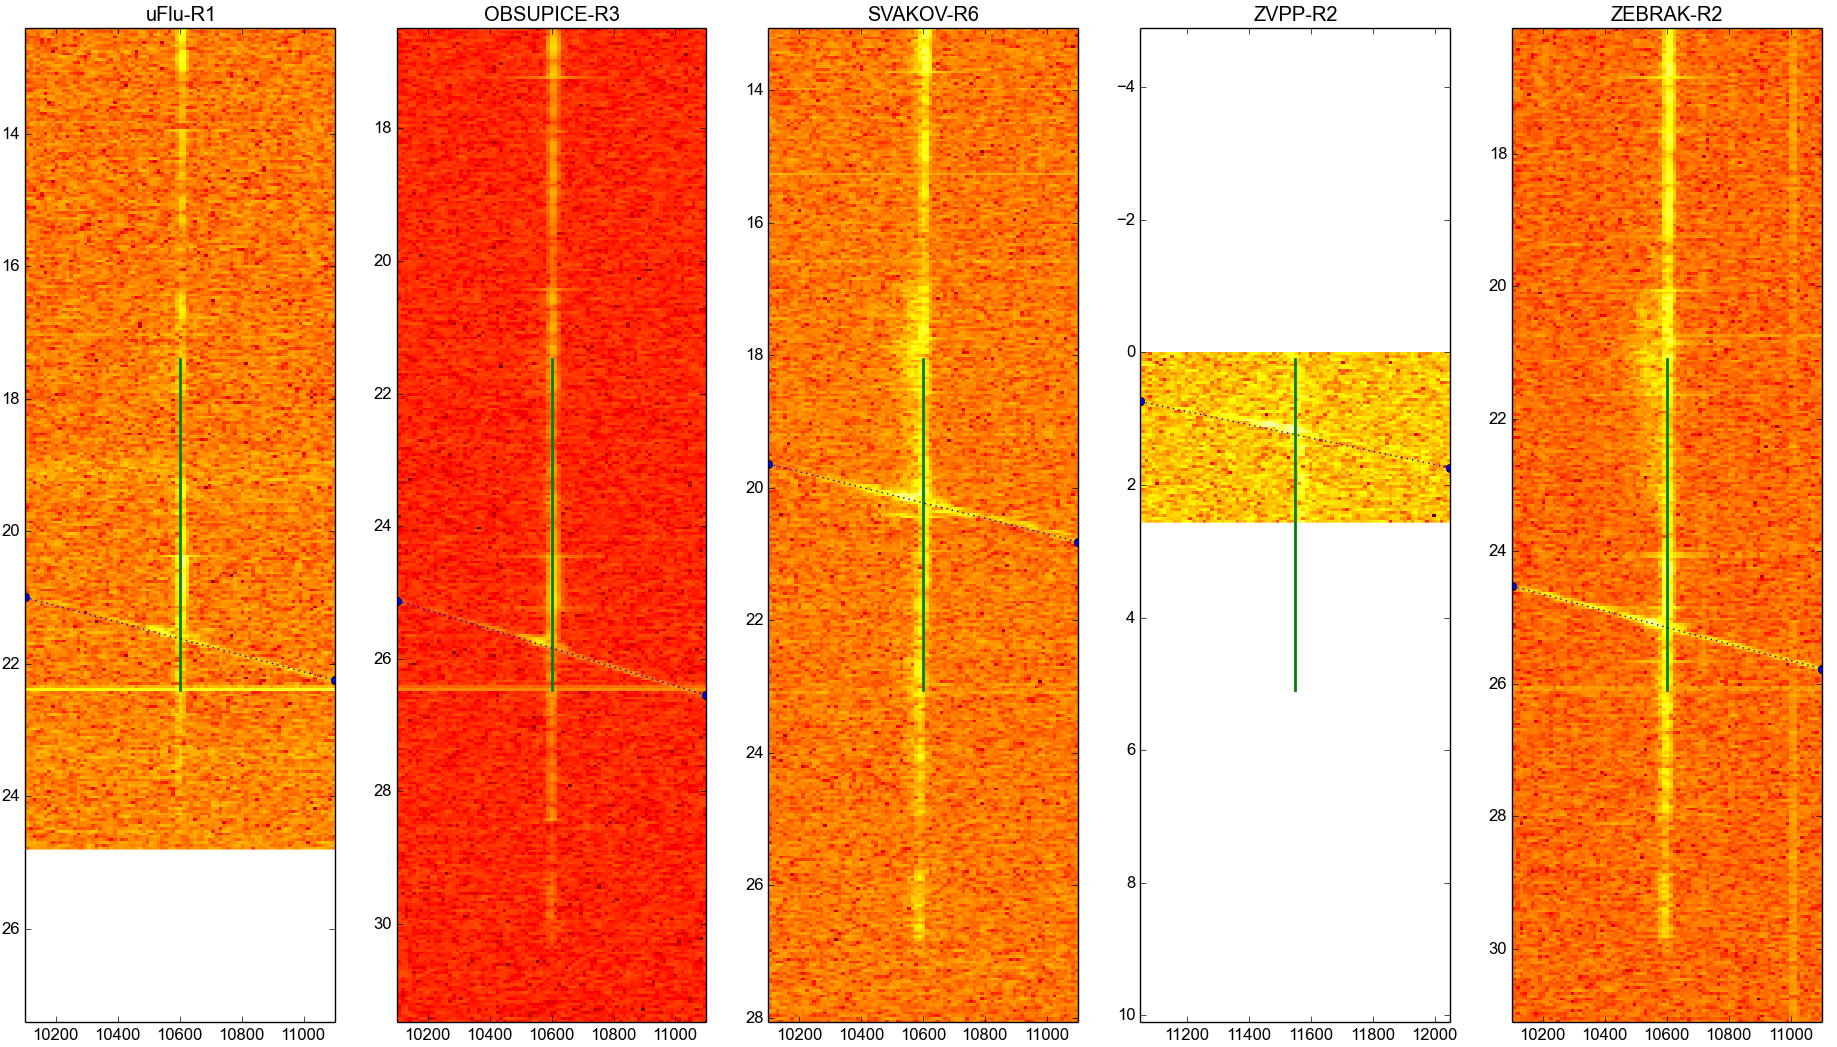
\includegraphics[width=\textwidth]{./img/Raws_analyser.png}
 \caption{Example of meteor reflections for multiple stations - Spectrograms show the time aligned signal evolution over vertical axis. (The oldest data being at the bottom) Horizontal axis corresponds to the frequency. (Highest frequency on the right)}
  \label{fig:meteor_reflections} 
 \end{center}
\end{figure*}

\begin{equation}
F_{obs} << f_{pe} =\frac{\sqrt{\frac{n_e e^2}{m \epsilon_0}}}{2 \pi}
\label{equ:plasma_frequency}
\end{equation}
\begin{itemize}
\item $n_e$ is the number density of electrons
\item $e$ is the elementary electrical charge
\item $m$ is the effective mass of the electron
\item $\epsilon_0$ is the permittivity of vacuum.
\end{itemize}

Obviously, not all parts of the meteor trail are observable from one station as the signal can be scattered to different directions non-specularly.
However, if we use multiple receiving stations, we greatly increase the sensitivity, because several stations could be located in the reflection spots. Therefore it demonstrates the value of having stations working as a cooperative detection network.
The network of stations has many advantages over a single transmitter - single receiver configuration. For example, it brings about robustness which allows operability even in a case that a part of the system is under a maintenance and therefore not functional.
                   
There also exist signal processing advantages, especially if we want to compute meteor parameters such as its velocity and trajectory from the meteor radio observation. All physical parameters we could determine from the single reflection are signal intensity and frequency shift in a given time which corresponds to an ionization intensity and bi-static velocity.
Therefore we must combine information about one meteor event from multiple stations to obtain points in space corresponding to the meteor trajectory. We align the events according to time stamps. Therefore, a precise time synchronization between the stations is required. The exact required precision depends on the network geometry. However, if we want to work in 300 m distance resolution, which is typical for the current optical methods, we need the time precision on approximately the microseconds scale. Therefore, we needed to develop a high-performance receiver with specific parameters, in particular with a high quality of time synchronization. Tight time synchronization requirements between nodes increase the complexity of the receiver system. To simplify the development process we used MLAB open source electronic prototyping platform \cite{Bolidozor},\cite{MLAB}.

As a result, a new type of radio meteor detection system is being built, based on a new idea of distributed scientific measurement systems. At the moment Bolidozor network produces a large volume of valuable radioastronomical data ready for further processing.  
We currently have an extensive database of multi-station meteor reflections. Unfortunately, we have yet not reached a suitable network geometry \cite{Positioning_geometry_Influence} to reliably obtain meteor position and trajectory by the known methods \cite{Doppler_method}. 
To overcome the missing algorithm issue, a further evolution of Bolidozor network should be focused on the research of the new trajectory estimation algorithms. We are also working on the network extension outside of GRAVES radar range with the aim of extending its service area as well as increasing the station's density which should decrease data noise and improve the numerical stability of algorithms. 

\subsection{VOR Transmitters as signal sources}
Although GRAVES military radar is a high power transmitter which easily allows basic detection of meteors, it is not an optimal system for meteor localization because it only has one transmitter, measurement method cannot be extended to the whole Earth, and the transmitted signal is not suitably modulated to allow a useful distance measurement.  Therefore several other available transmitters are investigated, such as FM radio transmitters or VOR beacons. 

For feasibility study of meteor detection based on VOR beacons, a numerical signal model has been created. The spectrum of modeled signal is shown in figure \ref{VOR_signal}.

\begin{figure}
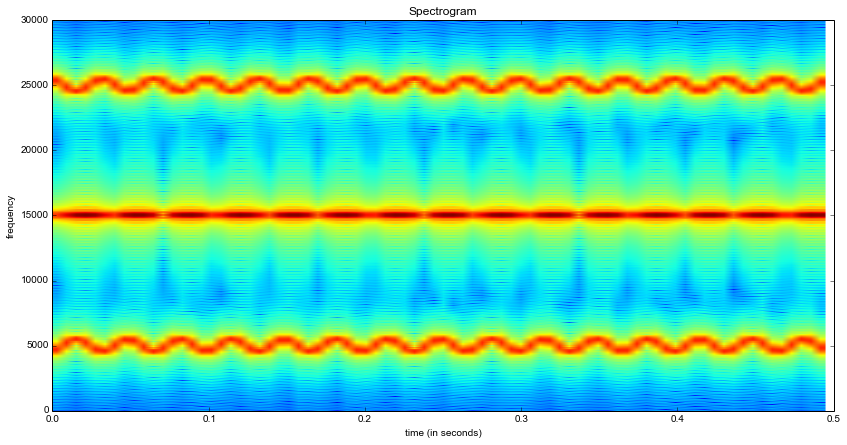
\includegraphics[width=\textwidth]{./img/VOR_signal.png}
\caption{VOR signal numerical model}
\label{VOR_signal}
\end{figure}

This signal is expected to be reflected from an ionized meteor trail, and signal reflection will be detected and extracted from the noise using the VOR signal replica. An intensity of received reflected signal was modeled by using a standard radar equation \ref{Radar_equation}.

\begin{equation}
P_r = \frac{P_t G_t G_r \lambda^2 \sigma}{(4 \pi)^3 R_t ^2 R_r ^2 L}
\label{Radar_equation}
\end{equation}
Where 
\begin{itemize}
\item $P_r$ — Received power in watts.
\item $P_t$ — Peak transmit power in watts.
\item $G_t$ — Transmitter antenna gain.
\item $G_r$ — Receiver antenna gain.
\item $\lambda$ — Radar operating frequency wavelength in meters.
\item $\sigma$ — Target's nonfluctuating radar cross section in square meters.
\item $L$ — General loss factor to account for both system and propagation loss.
\item $R_t$ — Range from the transmitter to the target.
\item $R_r$ — Range from the receiver to the target. 
\end{itemize}

The model generates many meteor trajectories (figure \ref{VOR_meteors} and calculates the signal power at receiver for point of closest approach. The resulting power histogram is shown in figure \ref{VOR_meteors_intensity}.

\begin{figure}
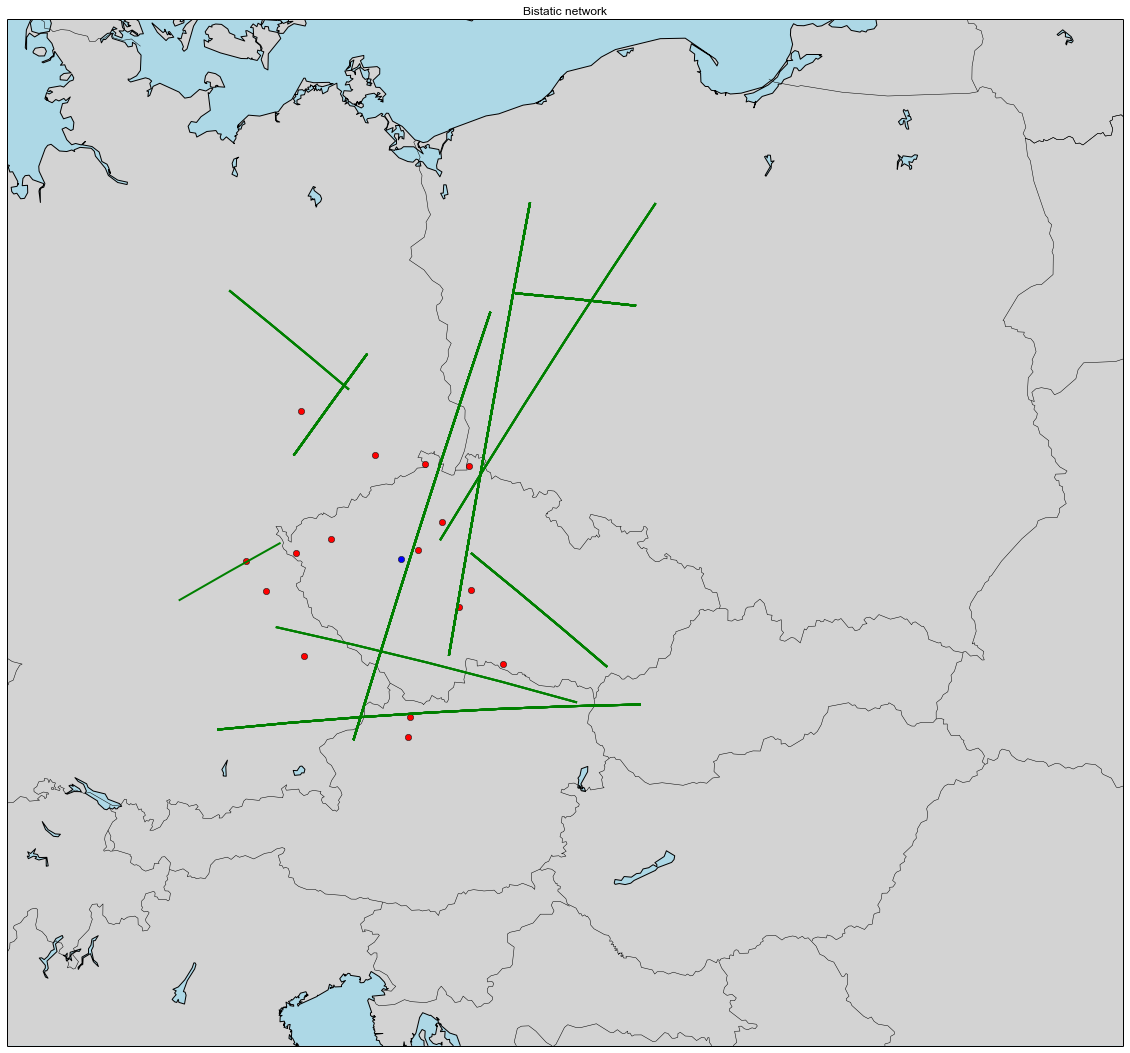
\includegraphics[width=\textwidth]{./img/Modeled_meteor_trajectories.png}
\caption{An example of random artificial meteor trajectories}
\label{VOR_meteors}
\end{figure}

\begin{figure}
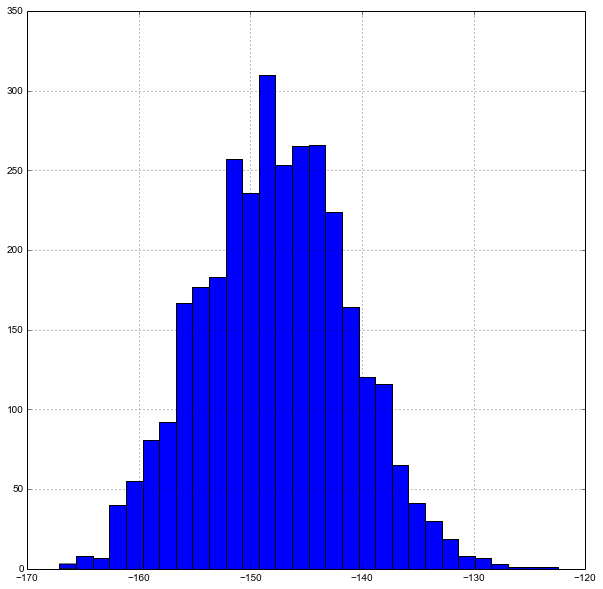
\includegraphics[width=\textwidth]{./img/Meteor_signal_intensity.png}
\caption{Distribution of expected signal power on receiver [dBm] on horizontal axis and meteor count on vertical axis.}
\label{VOR_meteors_intensity}
\end{figure}

As could be seen from resulting histogram, the power of expected received signal is on the verge of the radio receiver sensitivity. Therefore the detection could work over only a relatively small distance, and receiver system must therefore properly handle the strong ground signal and weak reflected signal. Such desired behavior could be probably best achieved by use of an antenna with suitable direction sensitivity.

\section{Hemispherical radiating pattern antenna design}

A highly directional pattern antenna is usually used for radio meteor observations, but these types of antennas became impractical in cases where we have multiple transmitters such as VOR beacons, spread around a reception station. In that situation, the hemispherical sensitivity and circular polarity uniformity of the antenna are more valuable than the peak directional antenna gain. A hemispherical radiation pattern antenna should be the best solution.  The symmetry of the radiation pattern of such antenna allows easy construction of antenna arrays which could be used for angular measurement of received signals.

\subsection{Patch Antenna Design }

Patch antenna was initially examined due to an expectation of a simple construction and easy manufacturing. The antenna was experimentally constructed from wire mesh with a square grid. This grid was chosen as a compromise between antenna quality (surface conductivity)  and the possibility of icing on antenna’s surfaces. Real prototype of the antenna was made according to the computer model. Unfortunately, after the antenna’s construction and verification, it was found that the antenna is very sensitive to deformation of patch base element and for a position of the central elevated element. Additionally, the central part must be a precise square to achieve a circular polarization. 

\subsection{Short-circuited quadrifilar helix}

Another antenna type was proposed to overcome the issues of the previous antenna design experiment.  Short-circuited quadrifilar helix (SC-QHA) is a variant of a well-known self-phased quadrifilar helix antenna (SP-QHA). However, unlike the SP-QHA type, the  SC-QHA has a narrower bandwidth which depends primarily on a bandwidth of a phasing network. Therefore the antenna could be more efficient for narrow band signals like meteor reflections.  The antenna was numerically modeled in NEC2++ software. See figures \ref{fig:QHA_antenna_RP}, which shows the expected radiation patterns of the antenna.  The prototype of the antenna was constructed based on the computer model, but a phasing network implementation becomes a challenging problem for practical usage of the SC-QHA antenna. 

\begin{figure*}
 \begin{center}
 \includegraphics[width=\textwidth]{./img/SC_QHA_prototype.jpg}
 \caption{A prototype of SC-QHA antenna which was build.}
  \label{fig:QHA_antenna} 
 \end{center}
\end{figure*}


\begin{figure*}
 \begin{center}
 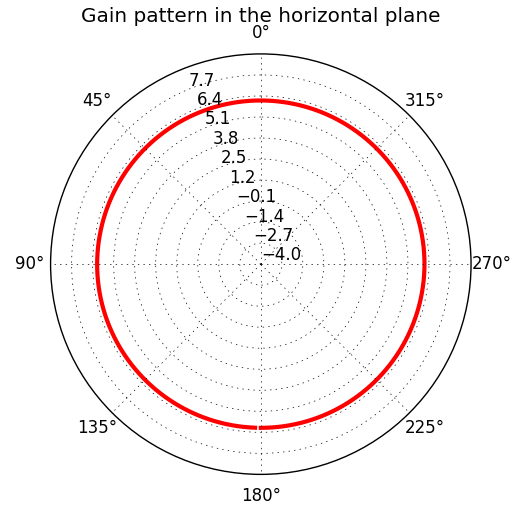
\includegraphics[width=90mm ]{./img/SC_QHA_rp_horizontal.png} 
 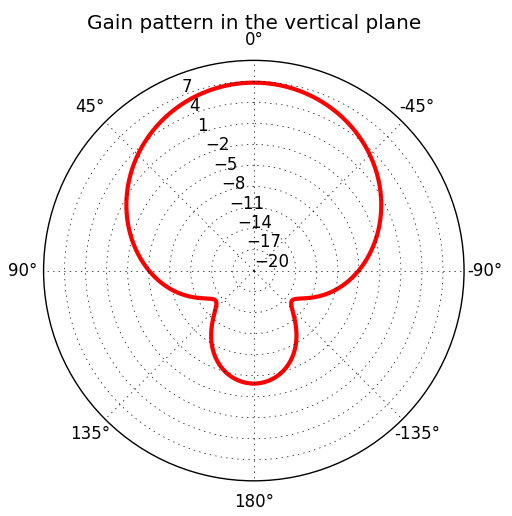
\includegraphics[width=90mm ]{./img/SC_QHA_rp_vertical.png}
 \caption{An expected radiation patterns generated by numerical antenna model.}
  \label{fig:QHA_antenna_RP} 
 \end{center}
\end{figure*}




\section{Meteor trajectory determination}

Every radio illuminated meteor trajectory in the atmosphere creates its Doppler shift reflection footprint which could be recorded by a network of receivers.  This process could be described by a numerical model of Doppler shifts for points on the trajectory. For simplicity, the tested model expects constant velocity along a straight line of the meteor path which is divided into equidistant time samples. A numerical difference of path distances between transmitter, meteor, and receiver are computed, then velocity and Doppler shift value are obtained for every point of the trajectory. 
The resulting figure of Doppler shifts calculated along the model meteor path radio-detectable on every existing station is shown in figure \ref{fig:dopplers}. 

\begin{figure*}
 \begin{center}
 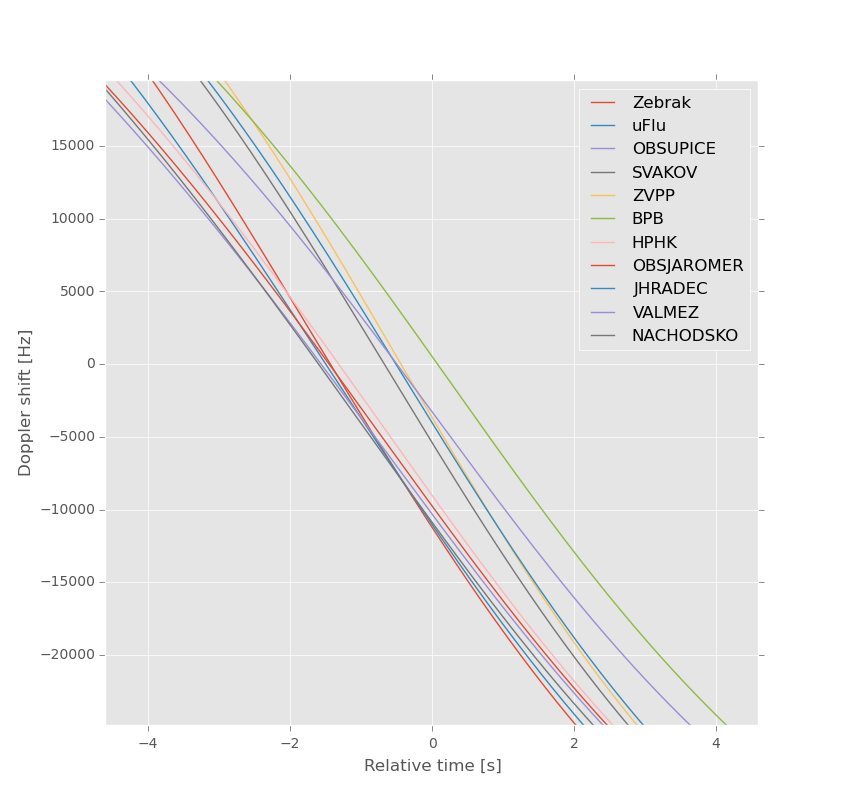
\includegraphics[width=\textwidth]{./img/Meteor_dopplers.png}
 \caption{Doppler shifts calculated for meteor ground path displayed in the figure \ref{fig:stanice_mapa}.}
  \label{fig:dopplers} 
 \end{center}
\end{figure*}


This signal model can be partially confirmed from Bolidozor meteor database where several meteor events are recorded on multiple stations. If we plot such meteor event in time aligned spectrogram, we obtain an image similar to the figure \ref{fig:meteor_reflections}.
Precise meteor trajectory estimation methods are investigated at the moment.  One of the difficulties is a possible suboptimal geometry configuration and low inter-station events coincidence.


\chapter{Future work}

Although some meteor trajectory estimation algorithms are developed, the real precision of estimation is unknown because it needs a comparison with other trajectory estimation method. The best candidate will be probably optical measurement performed at the event which is detected by radio method and by optical observations. A journal publication can be expected as the future result of this experiment. 

Algorithmic complexity of meteor trajectory estimation could be possibly reduced by introducing some additional information other than velocity measurements.  The direction finding using phased antenna array is the most promising candidate for improving the measurement method because a distance measurement is not usable for meteors due to the lack of a globally available network of transmitters which allows direct distance measurement.  However, distance measurement localization method could be used in the same system for natural phenomena which produce a wide-band time limited noise-like signal such as lightning.

\section{Expansion of used methods to other natural phenomena}

The analysis mentioned above of state of the art methods and systems leads to a conclusion that the dissertation should focus on multi-methodical detection and analysis of natural phenomena which is already the most promising area for radio scientific research. 
Already obtained experiences can be used for detection other natural phenomena like lightning strikes which could be extremely useful for work at the recently established CRREAT project which needs precise localization of atmospheric events to achieve its scientific goals. A publishable result could be expected according to CRREAT project roadmap because measurement of lightning position and its parameters are needed for describe the dependence on some other phenomena.  The CRREAT team will perform measurements of the atmospheric radiation and ionization events on satellites, aircraft, unmanned aerial vehicles, monitoring cars and ground stations. The CRREAT project will contribute to improvement of space weather models, air transport safety and global navigation systems reliability.

\section{Proposed lightning detection system}
The source \cite{LOFAR_lightning} suggests that the lightning pulses are strongly polarized where the polarization direction varies strongly for the individual peaks that form the total pulse. Combining the intensity and polarization information from many different antennas at different viewing angles on the discharge, the time structure, and direction of each charge movement can be determined.  This forms the input for building a 4-D vector map of the discharge current showing for every step the position in space as well as the direction of the electric current and therefore giving detailed insight into the spatiotemporal development of the lightning.  The shape of each pulse is related to the time-dependence and the distance over which the current flows.
This hypothesis verification is a primary challenge for future work because currently used TOA methods mentioned above allows computation of cloud of points only, but lightning should be described by vectors instead. There is a point where work already done on meteor detection should be used on lightning vectors computation and significantly improve the state of the art lightning location techniques by following steps: 

\begin{itemize}
\item Optimal detection and signal processing algorithm research.
\item A receiver parameters optimization like signal and antenna bandwidth optimization for reaching the best possible system precision.
\item Station deployment optimization
\end{itemize}

 The result of this improvement should be used for investigation of lightning and ionizing radiation relations which help to improve air traffic safety. 

\appendix

\begin{thebibliography}{99}

\bibliography{refs}
\bibliographystyle{plain}

\bibitem{Radar_basics}
Small and Short-Range Radar Systems,Gregory L. Charvat, CRC Press 2014,Pages 1–35, Print ISBN: 978-1-4398-6599-6,eBook ISBN: 978-1-4398-6600-9

\bibitem{lightning_dose1}
J. R. Dwyer, D. M. Smith, M. A. Uman, et. al.,
Estimation of the fluence of high-energy electron bursts produced by thunderclouds and the resulting radiation doses received in aircraft
\emph{JOURNAL OF GEOPHYSICAL RESEARCH, VOL. 115, D09206}, doi:10.1029/2009JD012039, 2010

\bibitem{lightning_dose2}
D. Petersen, M. Bailey, W. H. Beasley, J. Hallett,
A brief review of the problem of lightning initiation and a hypothesis of initial lightning leader formation
\emph{JOURNAL OF GEOPHYSICAL RESEARCH, VOL. 113, D17205}, doi:10.1029/2007JD009036, 2008

\bibitem{lightning_dose3}
T. Torii, M. Takeishi, T. Hosono,
Observation of gamma-ray dose increase associated with winter thunderstorm and lightning activity
\emph{JOURNAL OF GEOPHYSICAL RESEARCH, VOL. 107, NO. D17, 4324}, doi:10.1029/2001JD000938, 2002

\bibitem{lightning_dose4}
A Drozdov, A Grigoriev
Neutrons from thunderstorms at low atmospheric altitudes and related doses at aircraft
\emph{23rd European Cosmic Ray Symposium (and 32nd Russian Cosmic Ray Conference)}, doi:10.1088/1742-6596/409/1/012246

\bibitem{lightning_dose5}
A. Chilingarian
Thunderstorm Ground Enhancements (TGEs) - New High - Energy Phenomenon Originated in the Terrestrial Atmosphere
\emph{23rd European Cosmic Ray Symposium (and 32nd Russian Cosmic Ray Conference)}, doi:10.1088/1742-6596/409/1/012019

\bibitem{lightning_dose6}
K. B. Eack, W. H. Beasley
Long-duration X-ray emissions observed in thunderstorms
\emph{Journal of Geophysical Research: Atmospheres}, doi:10.1002/2015JD023262

\bibitem{BRAMS}
LAMY, H., ANCIAUX, M., RANVIER, S.,
Recent advances in the BRAMS network
\emph{Proceedings of the International Meteor Conference}, Mistelbach, Austria, 27-30 August 2015, Eds.: Rault, J.-L.; Roggemans, P., International Meteor Organization, ISBN 978-2-87355-029-5, pp. 171-175

\bibitem{NMLMA}
Rison, W., R.J. Thomas, P.R. Krehbiel, T. Hamlin, and J. Harlin, A GPS-based Three-Dimensional Lightning Mapping System: Initial Observations in Central New Mexico
\emph{Geophysical Research Letters, 26, 3573-3576, 1999}

\bibitem{LOFAR}
K. Mikhailov, J. van Leeuwen, 
The LOFAR search for radio pulsars and fast transients in M33, M81 and M82,
\emph{Astrophysics of Galaxies, A\&A 593, A21 (2016)}, DOI: 10.1051/0004-6361/201628348

\bibitem{LOPES}
F. G. Schröder, Instruments and Methods for the Radio Detection of High Energy Cosmic Rays,
\emph{DISSERTATION}, Tag der mündlichen Prüfung: 11. Februar 2011

\bibitem{LOFAR_showers}
Radio detection of air showers with LOFAR and AERA - LOFAR key science project Cosmic Rays and Pierre Auger Collaborations (Hörandel, Jörg R. for the collaboration) JPS Conf.Proc. 9 (2016) 010004 arXiv:1509.04960 [astro-ph.HE]

\bibitem{interplanetary_medium}
MANN, I., PELLINEN-WANNBERG, A., MURAD, E., et. al.
Dusty plasma effects in near earth space and interplanetary medium.
\emph{Space Science Reviews}, 2011, Vol. 161, Issue 1-4: 1-47 
10.1007/s11214-011-9762-3 

\bibitem{astro_particles}
J. Stasielak, R. Engel, S. Baur, P. Neunteufel, R. Šmída, F. Werner, H. Wilczyński
Feasibility of radar detection of extensive air showers
\emph{Astroparticle Physics}, Volume 73, 15 January 2016, Pages 14–27, astropartphys.2015.07.003 


\bibitem{Bland01102004}
BLAND, PHILIP, A.,
The Desert Fireball Network
\emph{Astronomy \& Geophysics}, vol. 45, number 5. pages 5.20-5.23
10.1046/j.1468-4004.2003.45520

\bibitem{RETRAM}
S. AZARIAN,J.J. MAINTOUX, F. RIBLE, J. MAINTOUX,
RETRAM: A network of passive radars to detect and 
track meteors
978-1-4799-4195-7/14/31.002014IEEE

\bibitem{light_pollution}
KAC, J.,
Meteor Observation and the Light Pollution
\emph{Proceedings of the International Meteor Conference}, Porec, Croatia, 24-27 September, 2009 Edited by Andreic, Z.;  International Meteor Organization, ISBN 2978-2-87355-022-6, pp. 68-75

\bibitem{skiymet}
HOCKINGA, W.K., SINGERB, W., BREMERB, J.,
Meteor radar temperatures at multiple sites derived with SKiYMET radars and compared to OH, rocket and lidar measurements
\emph{Journal of Atmospheric and Solar-Terrestrial Physics}
Volume 66, Issues 6-9, April-June 2004, Pages 585-593
doi:10.1016/j.jastp.2004.01.011

\bibitem{infrasound}
EDWARDS, W. N., BROWN, P. G., WERYK, R. J., et. al.
Infrasonic Observations of Meteoroids: Preliminary Results from a Coordinated Optical-radar-infrasound Observing Campaign
\emph{Earth Moon Planet} (2008) 102:221-229
DOI 10.1007/s11038-007-9154-6

\bibitem{Bolidozor}
J. Kakona, M. Kakona, M. Poviser, et. al.
Bolidozor radio meteor detection network
\emph{roceedings of the IMC} (Mistelbach, 2015)

\bibitem{IMPACT_sensor}
C.T. Mata, J.G. Wilson,
FUTURE EXPANSION OF THE LIGHTNING SURVEILLANCE SYSTEM AT THE KENNEDY SPACE CENTER AND THE CAPE CANAVERAL AIR FORCE STATION, FLORIDA, USA  
\emph{22nd International Lightning Detection conference} (2012) 

\bibitem{LOFAR_lightning}
O. Scholten, Ad van den Berg,
Lightning Research project (https://www.kvi.nl/~scholten/Lightning/KVI-ProjectDescription-crackling-v1.pdf)
\emph{KVI - Center for Advanced Radiation Technology, University of Groningen.} (KVI-CART) 

\bibitem{LOFAR_lightning2}
O.Scholten, S. Buitink,R. Dina, et. al.
Lightning Imaging with LOFAR
\emph{ARENA 2016} (DOI: 10.1051/epjconf/201713503003) 

\bibitem{NALMA_algorithms}
W. J. KOSHAK, R. J. SOLAKIEWICZ,R. J. BLAKESLEE, et. al.
North Alabama Lightning Mapping Array (LMA): VHF Source Retrieval Algorithm
and Error Analyses
\emph{JOURNAL OF ATMOSPHERIC AND OCEANIC TECHNOLOGY} (VOLUME 21) 

\bibitem{rocket_triggered}
J. D. Hill, J. Pilkey,M. A. Uman, et. al.
Correlated lightning mapping array and radar observations of the initial stages of three sequentially triggered Florida lightning discharges
\emph{JOURNAL OF GEOPHYSICAL RESEARCH: ATMOSPHERES} (, VOL. 118, 8460–8481, doi:10.1002/jgrd.50660, 2013) 

\bibitem{Transient_peak}
C. E. Livingstone,
An instrument for “real-time” measurement of the decaying edge of transient signals,
\emph{IEEE Transactions on Instrumentation and Measurement, vol. IM-25, no. 2, pp. 120-125, June 1976.} doi: 10.1109/TIM.1976.6312325

\bibitem{VLF_TOGA}
Richard L. Dowden,  James B. Brundell, Craig J. Rodger, 
VLF lightning location by time of group arrival (TOGA) at multiple sites
\emph{ournal of Atmospheric and Solar-Terrestrial Physics 64 (2002) 817–830}


\bibitem{4DLSS}
William P. Roeder, Jon M. Saul,
Four Dimensional Lightning Surveillance System:  Status and Plans  
\emph{22nd International Lightning Detection conference} (2012)

\bibitem{Lightning_locating}
Kenneth L. Cummins, Martin J. Murphy,
An Overview of Lightning Locating Systems: History, Techniques, and Uses, With an In-depth Look at 
the U.S. NLDN \emph{IEEE Transaction on Electromagnetic Compat
ibility} (4/15/2009)


\bibitem{CMOR_radar}
WEBSTER, A. R., BROWN, P. G., JONES, J., et. al.
Canadian Meteor Orbit Radar (CMOR)
\emph{Atmos. Chem. Phys.}, 4, 679-684, 2004
www.atmos-chem-phys.org/acp/4/679/
SRef-ID: 1680-7324/acp/2004-4-679

\bibitem{forward_scatter}
WISLEZ, J.-M.,
Forward scattering of radio waves off meteor trails
\emph{Proceedings of the International Meteor Conference}, Brandenburg, Germany, 1995, p. 99-117

\bibitem{daylight_shover}
CLEGG, J. A. ,HUGHES,  V. A. A., LOVELL, C. B., 
The Daylight Meteor Streams of 1947 May-August
\emph{Monthly Notices of the Royal Astronomical Society}, Vol. 107, p.369

\bibitem{Decay_time}
POOLE, L. M. G.,
Duration distribution of radio echoes obtained from underdense shower meteor trains
\emph{Smithsonian Contributions to Astrophysics}, Vol. 11, p.181

\bibitem{GRAVES_radar}
ALLEN, T.,
A GRAVES Sourcebook, Version of 2013-08-07
[Online] Cited 2016-1-23. Available at: http://fas.org/spp/military/program/track/graves.pdf

\bibitem{MLAB}
HORKEL, M., CHROUST, J., JANAS, M., et. al. 
MLAB - The Modular Laboratory project.
[Online] Cited 2016-1-23. Available at: http://www.mlab.cz/

\bibitem{SDR-widget}
STRAND-BERGESEN, B, et. al.
SDR-Widget interface
[Online] Cited 2016-1-23. Available at: https://github.com/borgestrand/sdr-widget

\bibitem{ghpsdr3}
MELTON, J.,
Ghpsdr3
[Online] Cited 2016-1-23. Available at: http://openhpsdr.org/wiki/index.php?title=Ghpsdr3

\bibitem{RMDS}
UNIVERSAL SCIENTIFIC TECHNOLOGIES, s.r.o.,  
Radio meteor detection station RMDS02D
[Online] Cited 2016-1-23. Available at: http://wiki.mlab.cz/doku.php?id=cs:rmds

\bibitem{CAS}
South Bohemian Czech astronomy society department
\emph{Czech astronomy society annual report 2015}
Pages 40-46

\bibitem{iPython}
PEREZ,GRANGER, F.,  BRIAN E.,
IPython: A System for Interactive Scientific Computing
\emph{Computing in Science \& Engineering}
2007, vol 9.,number 3,  Pages 21-29

\bibitem{Jupyter}
RAGAN-KELLEY, M., PEREZ, F., GRANGER, B., et al.,
The Jupyter/IPython architecture: a unified view of computational research, from interactive exploration to communication and publication.
\emph{American Geophysical Union}, Fall Meeting 2014
12/2014

\bibitem{scipy}
JONES E, OLIPHANT E, PETERSON P, et al.
SciPy: Open Source Scientific Tools for Python
2001-, http://www.scipy.org/ [Online; accessed 2016-03-07].

\bibitem{Doppler_method}
STEYAERT, C.,VERBELEN, F., et al.,
Meteor Trajectory from Multiple Station Head Echo Doppler Observations
\emph{WGN, the Journal of the IMO} 38:4 (2010)

\bibitem{RWIAOA}
F. Kong, J. Wang, N. Zheng, G. Chen and J. Zheng,
A robust weighted intersection algorithm for target localization using AOA measurements,
\emph{2016 IEEE Advanced Information Management, Communicates, Electronic and Automation Control Conference (IMCEC), Xi'an,}  2016, pp. 23-28. doi: 10.1109/IMCEC.2016.7867106

\bibitem{Interferometry_AOA}
F. Kong, J. Wang, N. Zheng, G. Chen and J. Zheng, 
A robust weighted intersection algorithm for target localization using AOA measurements,
\emph{2016 IEEE Advanced Information Management, Communicates, Electronic and Automation Control Conference (IMCEC), Xi'an,} 2016, pp. 23-28. doi: 10.1109/IMCEC.2016.7867106

\bibitem{TDOA_DP}
John D. Bard and Fredric M. Ham,
Time Difference of Arrival Dilution of Precision and Applications,
\emph{IEEE Transactions on Signal Processing, vol. 47, no. 2, pp.521-523, Feb. 1999}

\bibitem{Hyperbolic_location}
Y. T. Chan and K. C. Ho, 
A simple and efficient estimator for hyperbolic location,
\emph{IEEE Transactions on Signal Processing, vol. 42, pp. 1905–1915, Aug. 1994.}

\bibitem{Hyperbolic_accuracy}
Harry B. Lee, Accuracy Limitations of Hyperbolic Multilateration Systems,
\emph{IEEE Transacations on Aerospace and Electronic System, vol. AES-11, no. 1, pp.16-29, Jan, 1975}

\bibitem{GDOP}
N. Levanon,
Lowest GDOP in 2-D scenarios,
\emph{IEE Proceedings on Radar, Sonar and Navigation, vol 147, no. 3, pp. 149-155, June 2000}

\bibitem{GPS_GDOP}
R.Yarlagadda, l.Ali, N.Al-Dhahir and J.Hershey, 
GPS GDOP metric,
\emph{IEE Proceedings on Radar, Sonar and Navigation, vol. 147, no. 5, pp.259-264, October 2000}

\bibitem{Positioning_geometry_Influence}
K. Bronk, J. Stefanski, 
Bad Geometry Influence on Positioning Accuracy in Wireless Networks,
\emph{in EUROCON 2007 The International Conference on “Computer as a Tool”, Warsaw, pp.1131- 1135}

\bibitem{TOA_TDOA}
Dong-Ho Shin and Tae-Kyung Sung,
Comparisons of Error Characteristics between TOA and TDOA Positioning,
\emph{IEEE Transactions on Aerospace and Elcctronic ystems, vol. 38, no. 1, pp.307-311, Jan. 2002}


\end{thebibliography}

\end{document}